\section{Data structure}
\label{Sect:DataStructure}

{\bf Lead author:} Adam

The tracker data structure is shown in figure \ref{Fig:DataStructure} and is a subset of the overall MAUS data structure.  The basic unit of the MAUS data structure is the spill, representing the data produced by a single actuation of the MICE target.  All MAUS modules (mappers, reducers, etc.) act on one spill at a time.  The spill is then split in to two sides, Monte Carlo data and reconstructed data.  A key rule is that MC data must never be stored on the reconstruction side.


\begin{figure}[htb]
    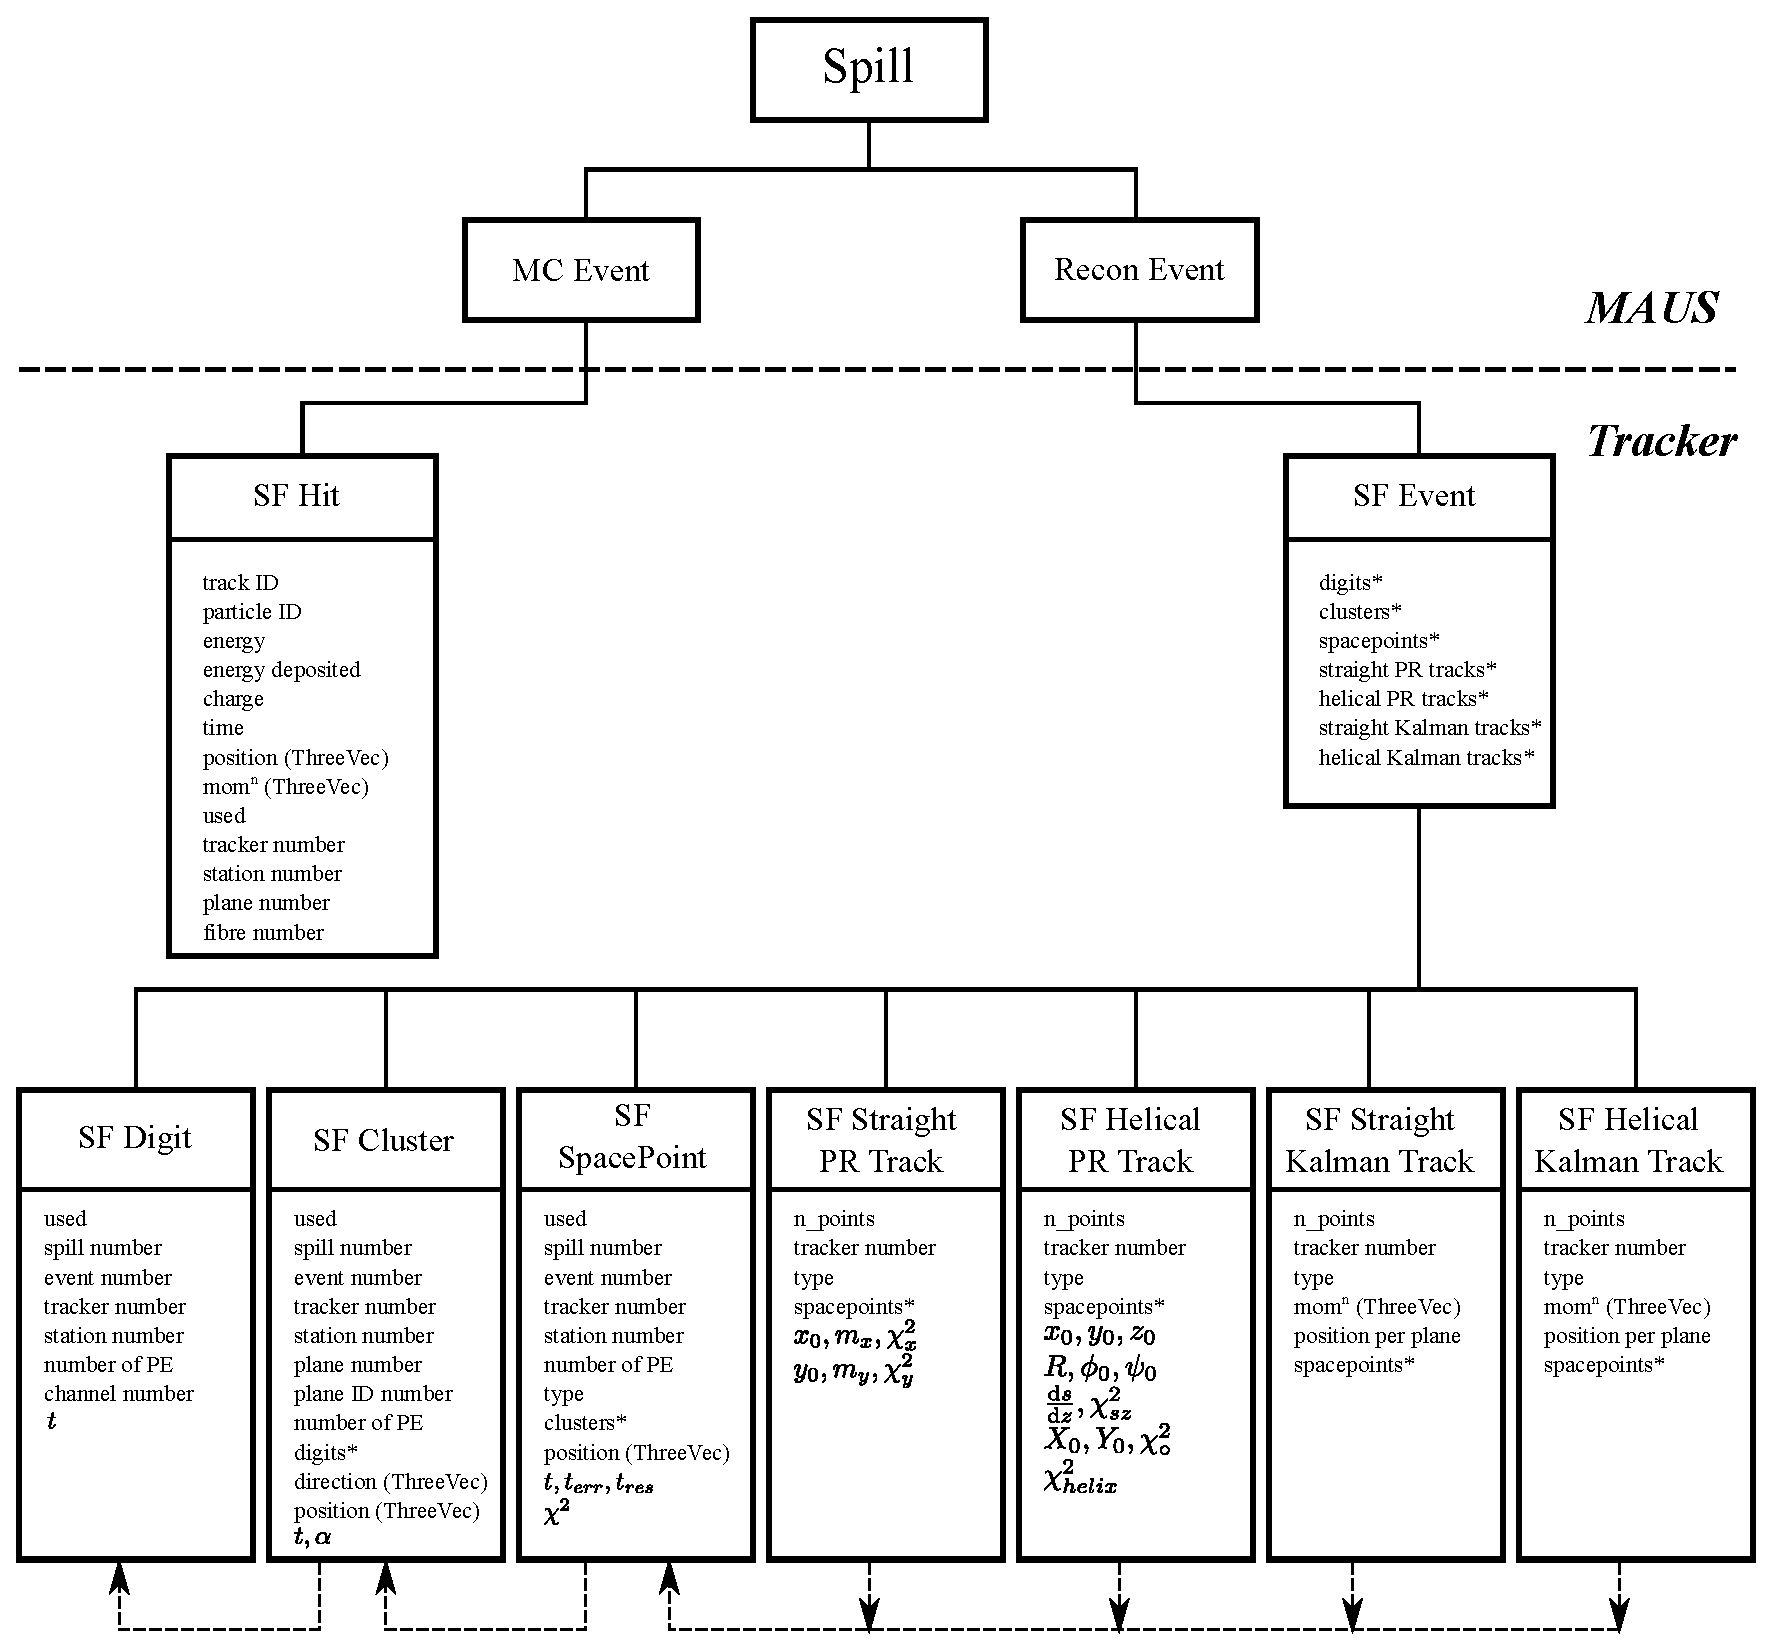
\includegraphics[width=0.85\textwidth]
      {05-DataStructure/Figures/DataStructure.eps}
    \caption{The tracker data structure and its position within the general MAUS data structure.}
    \label{Fig:DataStructure}
\end{figure}